\section{Quantification}

In order to perform a differential expression analysis, the expression of each
\gls{crna} needs to be quantified.
Multiple approaches to quantify \glspl{crna} have been introduced in
\cref{sec:crna_quantification}.
In the following, I will compare the quantification results of the detection
tools, multiple aggregations of the detection tools, and the quantification
tools.

\subsection{Comparison of quantification results}
\begin{figure}[ht] \begin{tabular}{cc} \begin{subfigure}{0.5\textwidth}
            \centering

            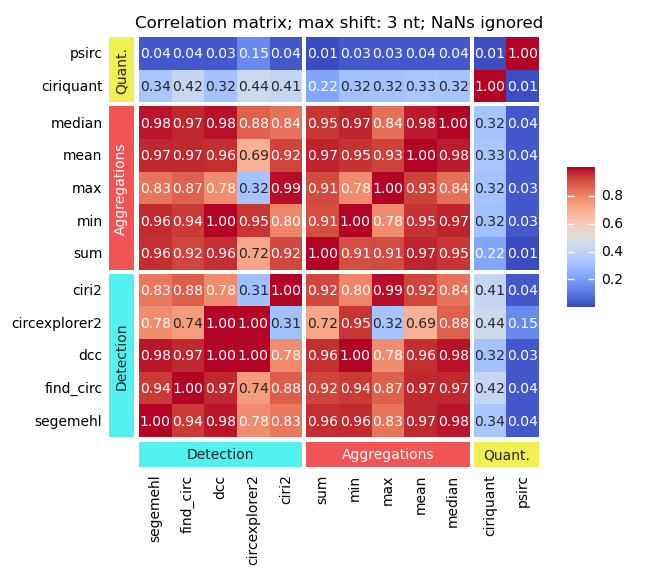
\includegraphics[width=\linewidth]{chapters/4_results_and_discussion/figures/quantification/correlation_heatmap_3_na.png}
            \caption{Missing values treated as \gls{nan}}
            \label{fig:correlation_heatmap_3_na}
        \end{subfigure} & \begin{subfigure}{0.5\textwidth} \centering

            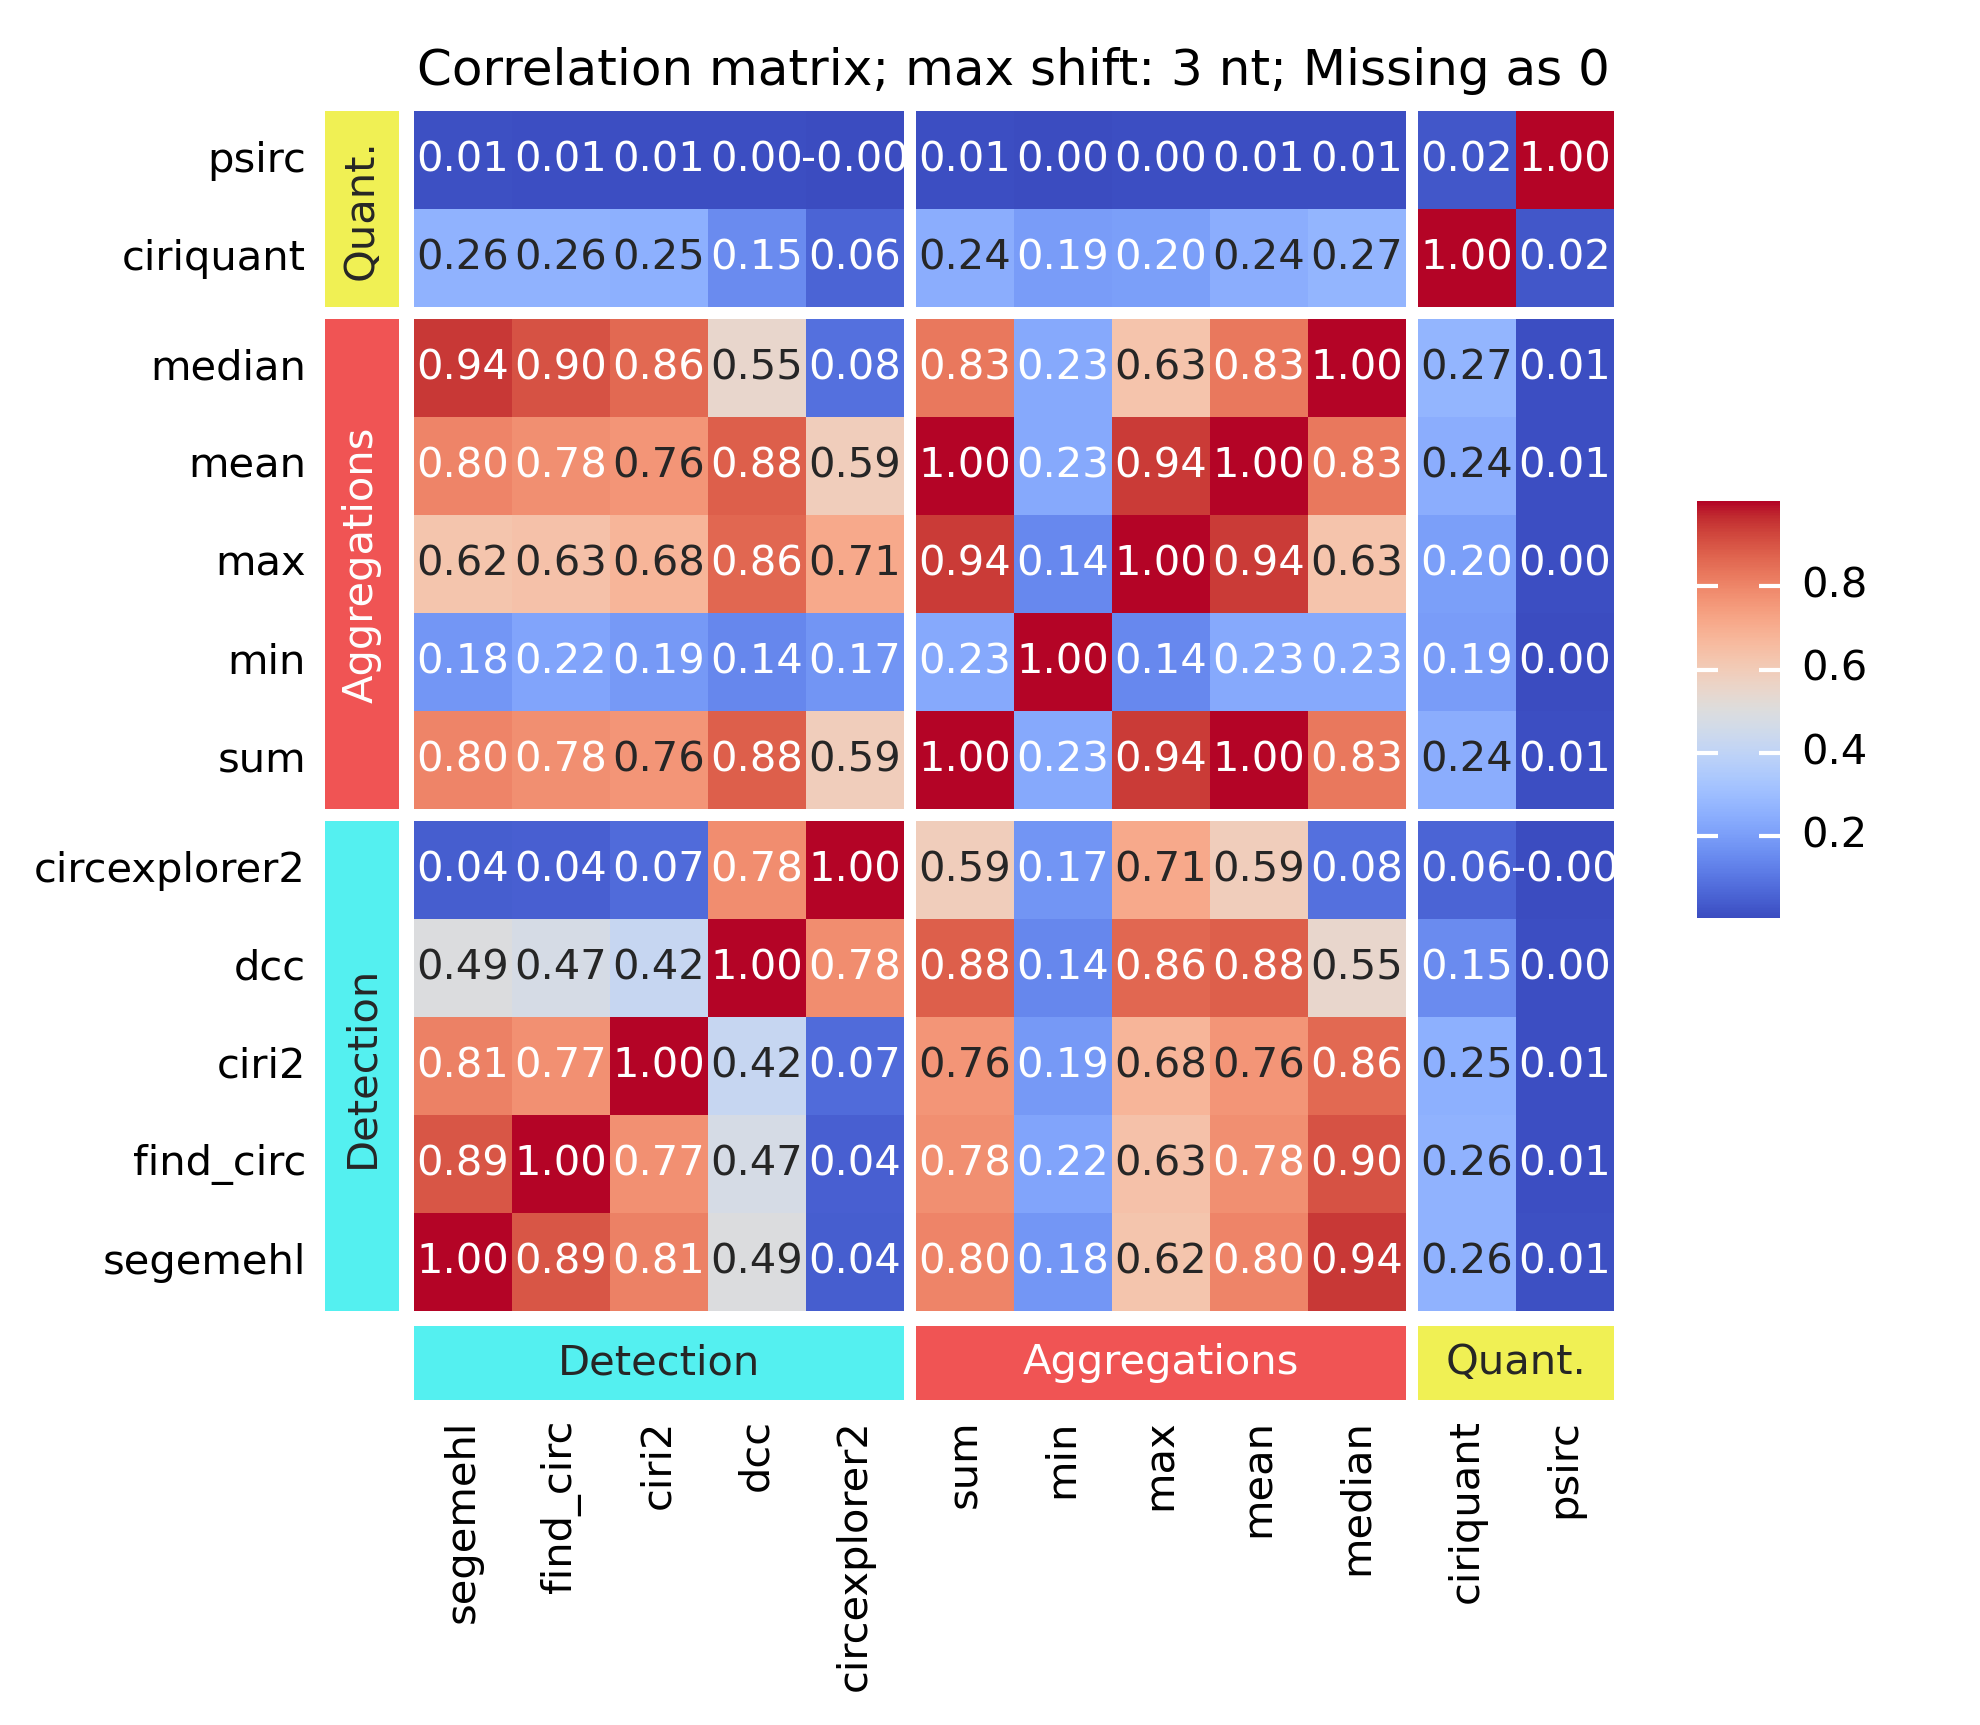
\includegraphics[width=\linewidth]{chapters/4_results_and_discussion/figures/quantification/correlation_heatmap_3_0.png}
            \caption{Missing values treated as 0}
            \label{fig:correlation_heatmap_3_0}
        \end{subfigure} \end{tabular} \caption{Pearson correlation heatmaps
        between the quantification results of the detection tools, multiple
        aggregations of the detection tools, and the quantification tools.
        The expression values were scaled so that the sum per sample and tool is
        constant.
        For each detected \gls{bsj}, expression information of all \glspl{bsj} within a
        \textit{max shift} of 3 on either strand was summed.
        \Cref{fig:correlation_heatmap_3_na} shows the correlation when treating
        missing values as \gls{nan}, while \cref{fig:correlation_heatmap_3_0}
        shows
        the
        correlation when treating missing values as 0.
    } \label{fig:correlation_heatmap} \end{figure}

As \cref{fig:correlation_heatmap} depicts, treating missing values as \gls{nan}
results in higher correlations overall.
However, treating the zeros as actual 0 values better reflects the underlying
biology.
This is because missing values mean that a tool did not detect any reads
supporting a \gls{bsj} (thus not outputting anything), which is equal to the
definition of 0 expression.

\subsubsection{Quantification tools}
Interestingly, the quantification tools show relatively low correlation with
the detection tools and aggregations.
While both show robust results in their respective publications, they were only
validated on paired end
data\supercite{zhang_accurate_2020,yu_quantifying_2021}.

\paragraph{\glsfmtlong{psirc-quant}}
For \gls{psirc-quant}, there is an additional complication: As mentioned in
\cref{sec:psirc}, it expects the \gls{fli} sequence as input.
As this study is based on single-end data, this information is not available.
Therefore, the entire sequence within the \gls{bsj} boundaries is used as the
\gls{crna} sequence.
While \gls{psirc-quant} uses the information that the sequence is circular when
constructing the \gls{t-dbg}, it does not treat reads spanning the \gls{bsj}
differently from reads that do not\supercite{yu_quantifying_2021}.

While due to the lack of ground truth it is impossible to say that the
quantification results of \gls{psirc-quant} are wrong, the low correlation with
the detection tools indicates that they are at least questionable in this
context.
Thus, I will not use the quantification results of \gls{psirc-quant} in the
following analyses.

\paragraph{\glsfmtlong{ciriquant}}
\Gls{ciriquant}, on the other hand, shows a higher correlation with
the detection tools and aggregations than \gls{psirc-quant}.
However, it is still relatively low ($<$0.35 in all comparisons when treating
missing values as 0).
Here, it is not clear why the correlation is so low, as \gls{ciriquant} uses a
similar approach to the detection tools.
Again, the lack of a ground truth makes it impossible to say whether the
quantification results of \gls{ciriquant} are trustworthy in this setting.

\subsubsection{Detection tools}
In \cref{fig:correlation_heatmap} it appears like there are two groups of
detection tools: One including \gls{segemehl}, \gls{findcirc} and \gls{ciri2},
and the other including \gls{dcc} and \gls{cex2}.
Both show high internal correlation in both settings ($>$0.7) and low
correlation between the groups ($\leq$0.55).

A potential explanation for the high correlation between \gls{cex2} and
\gls{dcc} is that they are both based on the same alignment generated by
STAR\supercite{dobin_star_2013}.
The other tools each use a different alignment method.
This however does not explain the high internal correlation between
\gls{segemehl}, \gls{findcirc} and \gls{ciri2}.

\subsubsection{Aggregations}
Many of the investigated aggregations seem to be able to smoothen out the
differences between the two groups of detection tools.
In the following paragraphs, I will look into the individual aggregations in
more detail.

\paragraph{min}
Using the minimum expression value of all tools for each \gls{bsj}
interestingly results in high correlations with \gls{findcirc} and
\gls{segemehl} when treating missing values as \gls{nan}.
In this setting, the minimum expression will be the smallest value of tools
with an expression value.
When looking at the behaviour of the min aggregation when treating missing
values as 0, we see that all correlation values are $<$0.25.
Here, the min aggregation will be 0 if any of the tools did not detect any
reads supporting a \gls{bsj}, which is true for many \glspl{bsj}.

\paragraph{median}
The median aggregation shows a tendency to correlate with the
segemehl-\gls{findcirc}-\gls{ciri2} group.
This is not surprising, as this group consists of 3 tools whereas the
\gls{dcc}-\gls{cex2} group consists of only 2 tools.
Thus, if all tools detect a \gls{bsj}, the median will be the lowest entry from
the first group.

\paragraph{max}
The max aggregation interestingly has high correlations with \gls{dcc} and \gls{cex2}
in the \gls{nan} setting.
This indicates that - if they detect a \gls{bsj} - they often detect a high
number of reads supporting it.
In the 0 setting, the max aggregation achieved a correlation $\geq 0.55$ with
all tools, thus yielding stable, but slightly worse results than the following
aggregations.

\paragraph{sum}
The sum aggregation results in robust correlations in both settings.
While the correlation with \gls{cex2} is lower than with the other tools in the
0 setting, this is mostly due to the fact that \gls{cex2} detects fewer
\glspl{bsj} than the other tools.
This is supported by the fact that \gls{cex2} has a high correlation of 0.96 in
the \gls{nan} setting, where only \glspl{bsj} where \gls{cex2} detected reads
are considered.

\paragraph{mean}
This behaves very similarly to the sum aggregation.
Mathematically, the mean aggregation is the sum divided by the number of tools
with an expression value.
Thus, in the 0 setting, they are equal, while in the \gls{nan} setting, the
mean aggregation will deviate if a tool did not detect any reads supporting a
\gls{bsj}.

\subsection{Conclusion}

While \gls{psirc-quant} appears to be unsuitable for quantification if the
\gls{fli} sequence is not available, \gls{ciriquant} at least shows some
correlation with the detection tools and aggregations.
As there is no ground truth available, both the sum aggregation and the
quantification results of \gls{ciriquant} will be considered in the following
analyses.
